 \section{Background}
Control Systems broadly come in two flavours: \textit{Open-loop} systems and \textit{Closed-loop} systems. Open-loop systems are systems which take in an input and execute it as perfectly as possible without any capability of inferring if the execution went as intended. The primary drawback of open-loop system is that it requires a perfect mathematical model of the complete system and its surrounding environment. Thus, open-loop systems work only in simple cases where it is easy to model all the factors that affect the output of the control system. In practice however, this is rarely the case. As a result, engineers have turned to closed-loop systems which have a feedback element that is used to minimize the error between the desired mission and the actual mission being executed. This is necessary since it is impossible to perfectly model beforehand the vagaries of the external disturbances as well as the noise inherent in the system.

A schematic diagram of a closed-loop system is shown in Figure \ref{fig:control system}.

\begin{figure}
    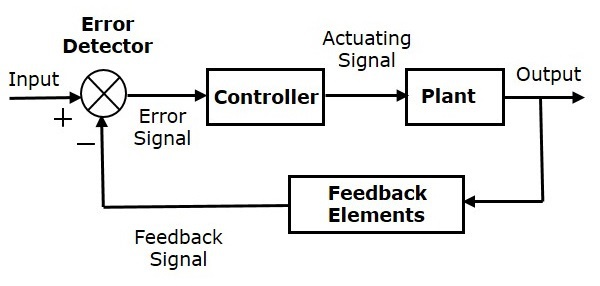
\includegraphics[scale=0.40]{images/closed_loop.jpg}
    \caption{Schematic diagram of a Control System}
    \label{fig:control system}
\end{figure}


As described in the figure, a general closed-loop system has 4 components:

\begin{itemize}
    \item \textit{Controller:} Controller is a component that takes in the sensor values and converts it into control commands $z_k$ that is to be sent to the actuators. For example, the controller could be a PID controller that estimates and keeps track of position. We could have similar controller to provide feedback-based control to attitude(roll, pitch and yaw) of a UAV.
	\item \textit{Plant or Process:} The physical phenomena of interest, called the physical environment. For example, the position of a UAV or the acceleration of a UAV. The controller's task is to moderate the plant and steer it to the desired output. The controller accomplishes this using actuators. Actuators are components that executes the control commands sent by the controller. Typically, actuators are components such as motors and propellers that causes a change in physical environment around the CPS.
	\item \textit{Feedback Elements:} These are components which sense the outputs driven by the controllers and transmits it in a time-series, denoting the measurement of physical environment at every time instance. For example, the GPS sensor or accelerometer in a UAV is a sensor that sends in time series of position values to the controller.
 

\end{itemize}

\textbf{Cyber-Physical Systems(CPS)} CPS's are examples of closed loop systems, since, the physical subsystem executes commands from the computing system and the the computing subsystem consumes the sensor values perceived by the physical subsystem. Typically a physical subsystem consists of a combination of sensors and actuators. These two subsystems are connecting to form a feedback-based control system as shown in Figure \ref{fig:cps}

\begin{figure}
    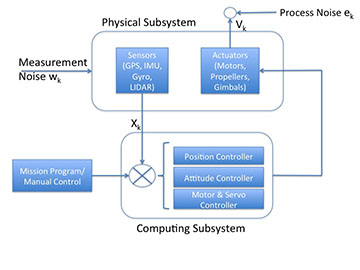
\includegraphics[scale=0.60]{images/cps-fig-small.jpg}
    \caption{Schematic diagram of a Cyber-Physical System}
    \label{fig:cps}
\end{figure}
%Insert picture of a cyber-physical system here with both cyber and physical aspects

As Figure \ref{fig:cps} describes, there are cyber and physical realms that are feedback control with one another. The mission control program could be as simple as preset waypoints on a map or it could be as complex as a neural network taking multiple inputs. In the case of a UAV, it could be something external such as manual commands using radio controller joystick to drive the UAV.  There are two kinds of noise that are in play here. First is the measurement noise, which gets mixed with the sensors while a measurement of the physical environment is obtained. In short, this noise accounts for imperfection in measurements and is typical in all measurement-based systems. Second is the process noise, which gets mixed with the environment when the controller drives the outputs to physical environment. In other words, this noise accounts for imperfect actuation.

\subsection{Attacks on CPS Systems}
There are multiple ways to compromise a CPS system. However, we would be generalizing the attacks into three broad categories. First, the attack could be on one of the actuators. This is typically done by intercepting the control command executed by the actuator to effect the physical environment around the CPS. In other words, the control command executed differs wildly from $v_k + e_k$ as it should be from Figure \ref{fig:cps}. This could result from the actuation mechanism itself being compromised or by accepting a control command from an untrusted agent. This false actuation will affect the measured variables of the physical environment and thereby the sensor measurements are also tampered.

Second, the attack could be on the sensors in the system. This is typically done by altering the perception of the physical environment around the CPS system. As a result, the sensor measurement used by the controller would be different from the real state of the measured variables. In other words, the physical process being measured differs wildly from $x_k + w_k$. Similar to attacks on actuators, attacks on sensors have the effect of circulating in the closed loop system, once injected.

Third, and perhaps the most grievous, is the case of the controller device getting compromised as well, giving the attacker unlimited control to implement any outcome. To detect this, one would need an unbiased view of the CPS system from an external vantage point that could be a trusted ground control station or a trusted UAV to perceive the state and compare it with the monitored UAV. 

In this paper, we are primarily concerned with attacks of the first two types of attacks -- attacks on actuators and sensors. We would be focusing on the design on a control-invariant framework that can help detect the attacks described. At a high level, our framework takes in measurements, say from sensors, $x_k$ and control commands, $V_k$  that are pushed out by the controller to the actuator and makes a binary decision of an attack via an anomaly detection technique. It is important to note that the idea of monitoring sensor measurements and control commands to identify issues with sensors, actuators or controllers is not a novel idea and is a popular idea in fault detection research. However, this style of fault detection relies on physical as well as spatial diversity (the technique of having multiple sensors or controllers and decide on majority voting) or functional redundancy(eg., measure a quantity directly as well as indirectly -- such as position being measured by double integrating acceleration). Furthermore, this sort of detection is not sufficient for an attacker, since, the effort to compromise multiple sensors having one compromised is O(1) -- via attack reuse.



